\chapter{Position and Orientation}\label{ch:position_rotation}

As it has been shown before, once the threshold segmentation has been applied to our cropped image from the workspace, the picture will look something of this sort:

\begin{figure}[hb]
  \centering
  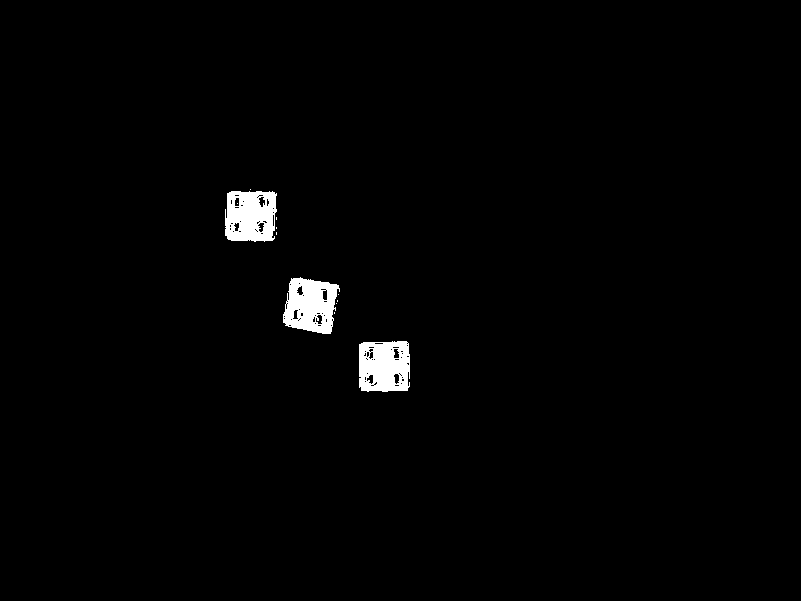
\includegraphics[width=4in]{figures/thresh_img.png}
  \caption[thresholded_image] {RGB Segmented Image}
\end{figure}


\subsection*{Orientation}
Besides the position, the measure of the required angle to turn the gripper is also essential to achieve the goal. Nevertheless, the coordinates of the center will be important to find the orientation of the bricks. 

First, four furthest points with respect to the center are necessary to find the coordinates of the corners. However, this search needs to be constrainted to ensure that the distance between each point is, at least, fifteen pixels, to avoid having more than one point in each corner.

Then, two of the previous corners are chosen in order to define one side of the square. The connection between these two corners and the center generates two different straight lines (from each corner to the center). Using the image with the edges of the desired block it was evaluated which points were below the generated lines. To finish this step, a linear regression was calculated and the parameters of the straight line were found.

Finally, the slope was converted to an angle to obtain the orientation of the brick. However, if the angle was negative it was necessary to calculate the one associated with the perpendicular line in order to have the correct orientation.
